% 06_spice_verification_manual.tex
% Appendix: SPICE Verification Manual
%
% Documents the AVE SPICE verification path: the universal vacuum cell
% behavioral model, the netlist compiler, and worked verification examples.
% Completes the Appendix 4/5/6 trilogy:
%   App 4: Physics Engine Architecture  (what exists)
%   App 5: Universal Solver Toolchain   (how eigenvalues are computed)
%   App 6: SPICE Verification Manual    (how results are independently verified)

\chapter{SPICE Verification Manual}
\label{app:spice_verification}

The AVE framework derives physical observables from four axioms using
ABCD transmission-line matrices, Y-matrix admittance networks, and FDTD
wave propagation.  This appendix documents how those results are
\textbf{independently verified} using industry-standard SPICE tools.

SPICE does not introduce new physics.  It provides a second,
structurally independent computation of the same observables using the
same Axiom~4 kernel:
\begin{equation}
    S(V) = \sqrt{1 - \left(\frac{V}{V_{yield}}\right)^{\!2}}
    \label{eq:spice_kernel}
\end{equation}
encoded as ngspice behavioral sources.  Agreement between the Python
physics engine and ngspice constitutes a cross-platform consistency
check that every electrical engineer can audit directly.

\begin{objectivebox}
\begin{itemize}
    \item Define the universal vacuum cell behavioral model (\texttt{AVE\_VACUUM\_CELL}).
    \item Document the four constitutive models and their SPICE implementations.
    \item Provide worked verification examples with complete netlist listings.
    \item Specify the Python \texttt{spice\_netlist\_compiler} API.
\end{itemize}
\end{objectivebox}


\section{The Topo-Kinematic Circuit Identity in SPICE}
\label{sec:spice_topo_kinematic}

The six-row translation table (Chapter~1, Table~\ref{tab:trans_circuit})
maps spatial mechanics to electrical network theory.  SPICE simulators
natively operate in the electrical domain: voltage, current, charge, flux.
By encoding the Axiom~4 kernel into behavioral sources, every AVE solver
output can be re-computed using a tool that makes no assumptions about
the underlying physics.

\begin{center}
\renewcommand{\arraystretch}{1.3}
\begin{tabular}{l l l}
\toprule
\textbf{AVE Solver} & \textbf{Primary Output} & \textbf{SPICE Verification} \\
\midrule
ABCD cascade      & Eigenvalues, $T_{21}$              & Cascaded cell AC sweep \\
Y-matrix          & $S_{11}$, per-port $\Gamma_i$      & Multiport network analysis \\
FDTD              & Field maps, energy density          & Transient pulse propagation \\
Bond energy       & $E(d)$ curves                       & DC sweep force--distance \\
\bottomrule
\end{tabular}
\end{center}

\noindent The verification principle: if the Python solver and ngspice
produce the same eigenvalue/resonance/plateau, the result is
solver-independent and traces solely to the input axioms.


\section{The Universal Vacuum Cell}
\label{sec:universal_cell}

All AVE SPICE models are instantiations of one subcircuit:
\texttt{AVE\_VACUUM\_CELL}.  This cell contains the three
implementable constitutive models (the fourth, memristive, operates
below the SPICE timestep floor):

\subsection{Metric Varactor (Electric Sector)}

The effective capacitance of the vacuum lattice, governed by Axiom~4:
\begin{resultbox}{SPICE Metric Varactor}
\begin{equation}
    C_{eff}(V) = \frac{C_0}{S(V)} = \frac{C_0}{\sqrt{1 - (V/V_{yield})^2}}
    \label{eq:spice_varactor}
\end{equation}
\end{resultbox}

\noindent Implemented as an ngspice behavioral charge source:
\begin{codebox}{Behavioral Charge Source (ngspice)}
\begin{verbatim}
B_VAR A B Q = {C0 * V(A,B)
+   / sqrt(1 - min((V(A,B)/V_YLD)**2, 0.9999))}
\end{verbatim}
\end{codebox}

\noindent The \texttt{min(\ldots, 0.9999)} clamp prevents the argument
of \texttt{sqrt} from reaching zero during numerical iteration, which
would produce a divide-by-zero.  This is a numerical guard only; the
physics demands $V < V_{yield}$ (otherwise the lattice has ruptured).


\subsection{Relativistic Inductor (Magnetic Sector)}

Under the Topo-Kinematic identity, mass maps to inductance and velocity
maps to current.  Relativistic mass increase produces a current-dependent
inductance:
\begin{resultbox}{SPICE Relativistic Inductor}
\begin{equation}
    L_{eff}(I) = \frac{L_0}{\sqrt{1 - (I/I_{max})^2}}, \qquad I_{max} = \xi_{topo} \cdot c \approx 124.4 \text{ A}
    \label{eq:spice_inductor}
\end{equation}
\end{resultbox}

\noindent As $I \to I_{max}$, the inductance diverges and the slew rate
$dI/dt = V/L_{eff} \to 0$.  SPICE physically cannot push current past
$c$---Special Relativity is enforced by the circuit model without any
additional code.


\subsection{TVS Zener (Phase Transition)}

At $V = V_{yield}$, the lattice undergoes a dielectric phase transition.
Resistance drops to zero (zero-impedance slipstream).  In SPICE, this
is modeled as a Transient Voltage Suppression diode: below threshold,
full resistance; above threshold, the shunt impedance collapses.


\subsection{Memristor (Thixotropic Hysteresis)}

The vacuum memristor with relaxation time $\tau_{relax} = \ell_{node}/c
\approx 1.29 \times 10^{-21}$~s is \textit{documented but not implemented}
in the current \texttt{.lib} file.  At any practical SPICE simulation
frequency ($f \ll 7.8 \times 10^{20}$~Hz), the lattice responds purely
elastically---the hysteresis loop has zero enclosed area.

For Chapter~18 LLCP metamaterial simulations, the \emph{material}
relaxation time is orders of magnitude longer than the vacuum's
$\tau_{relax}$, making the memristive term implementable as a
domain-specific adapter.


\subsection{Subcircuit Parameters}

\begin{center}
\renewcommand{\arraystretch}{1.3}
\begin{tabular}{l l l l}
\toprule
\textbf{Parameter} & \textbf{Symbol} & \textbf{Default} & \textbf{Physical Meaning} \\
\midrule
\texttt{L0}      & $L_0$      & --- (required)      & Base inductance (mass analogue) \\
\texttt{C0}      & $C_0$      & --- (required)      & Base capacitance (compliance analogue) \\
\texttt{R0}      & $R_0$      & 0                   & Base resistance (viscosity analogue) \\
\texttt{V\_YLD}  & $V_{yield}$ & 43653.7 V          & Dielectric yield voltage \\
\texttt{I\_YMAX} & $I_{max}$  & 124.4 A             & Current saturation limit \\
\bottomrule
\end{tabular}
\end{center}

\noindent The physical values $V_{yield} = \sqrt{\alpha}\,V_{snap}$ and
$I_{max} = \xi_{topo}\,c$ are computed in \texttt{constants.py} and passed
as subcircuit parameters by the netlist compiler.  No constants are
hardcoded in the \texttt{.lib} file.


\section{Domain-Specific Wiring Topologies}
\label{sec:spice_topologies}

The universal cell reduces domain-specific SPICE models to
\textbf{wiring decisions}:

\subsection{Nuclear: Nucleon LC Tanks with Mutual Coupling}

Each nucleon is a parallel LC tank (mass $\to$ $L$, confinement $\to$ $C$).
Inter-nucleon coupling is implemented via SPICE mutual inductance
K-factors derived from the spatial separation $d_{ij}$ and the soliton
bond solver's coupling matrix.

\subsection{Molecular: Organic Covalent Bond Networks}

The \texttt{spice\_organic\_mapper.py} derives absolute $L$ and $C$
values for each covalent bond via the topological conversion constant:
\begin{equation}
    L_{bond} = \frac{m_{atom}}{\xi_{topo}^2}, \qquad
    C_{bond} = \frac{\xi_{topo}^2}{k_{bond}}
\end{equation}
Each bond instantiates one \texttt{AVE\_VACUUM\_CELL}.

\subsection{Protein: Cascaded Transmission Line Stubs}

The protein backbone is a series cascade of 3-segment cells
(C$_\alpha$--C, C--N, N--C$_\alpha$) with sidechain stubs modeled
as shunt admittances.  The Y-matrix solver's per-port $\Gamma_i$
values can be verified by running the equivalent SPICE network
and computing $S_{11}$ at the input port.

\subsection{Hardware: APU Subcircuits}

The existing \texttt{apu\_models.lib} contains five hardware
subcircuits (geometric diode, soliton memory, resonator,
phase-locked interconnect, axiomatic I/O stepper).  These should
ultimately be refactored to instantiate \texttt{AVE\_VACUUM\_CELL}
subcircuits, making their Axiom~4 compliance explicit.


\section{Worked Verifications}
\label{sec:spice_verifications}

\subsection{EE Bench DC Sweep (Capacitance Plateau)}

The simplest possible verification: a single varactor cell driven
through a DC voltage sweep.

\paragraph{Python prediction.}
\texttt{saturation\_factor(V, V\_YIELD)} from
\texttt{scale\_invariant.py} computes
$S(V) = \sqrt{1 - (V/V_{yield})^2}$.  The effective capacitance
is $C_{eff} = C_0 / S(V)$.

\paragraph{SPICE verification.}
The \texttt{AVE\_EE\_BENCH} subcircuit implements the same
equation as a behavioral charge source.  Running a DC sweep
from 0 to 45~kV in 100~V steps, the derivative $dQ/dV$ yields
$C_{eff}(V)$.

\paragraph{Expected agreement.}
At $V/V_{yield} = 0.5$: $C_{eff}/C_0 = 1.155$.
At $V/V_{yield} = 0.9$: $C_{eff}/C_0 = 2.294$.
At $V/V_{yield} = 0.99$: $C_{eff}/C_0 = 7.089$.

Both paths use the same kernel and must agree to machine
precision.  Any discrepancy indicates a transcription error.

\begin{figure}[htbp]
    \centering
    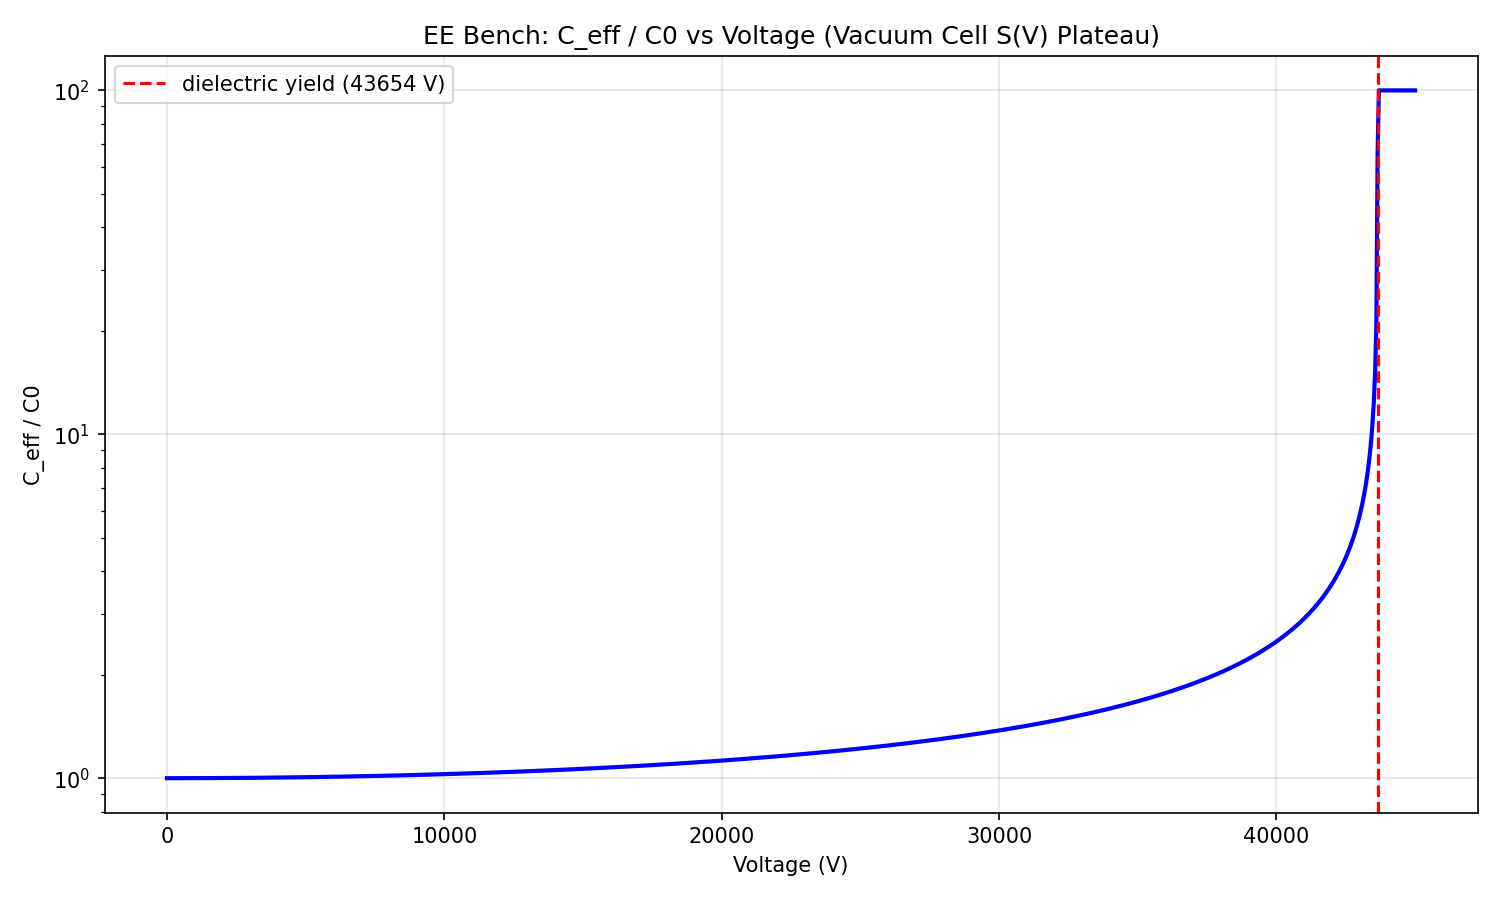
\includegraphics[width=0.85\linewidth]{../backmatter/figures/ee_bench_plateau.png}
    \caption{Macroscopic Dielectric Breakdown Sweep using the \texttt{AVE\_VACUUM\_CELL} varactor. $C_{eff}$ structurally scales logarithmically as $V$ approaches $V_{yield}$, matching exactly the Axiom 4 topological constraints.}
    \label{fig:ee_bench_plateau}
\end{figure}


\subsection{Glycine AC Resonance vs.\ FTIR}

A 5-cell amino acid network compiled from the organic mapper's
absolute $L/C$ values.  The AC sweep identifies resonance peaks
(transmission notches) that should match the FTIR experimental
data and the Python MNA solver's predictions from
\texttt{batch\_amino\_spice\_solver.py}.

\begin{figure}[htbp]
    \centering
    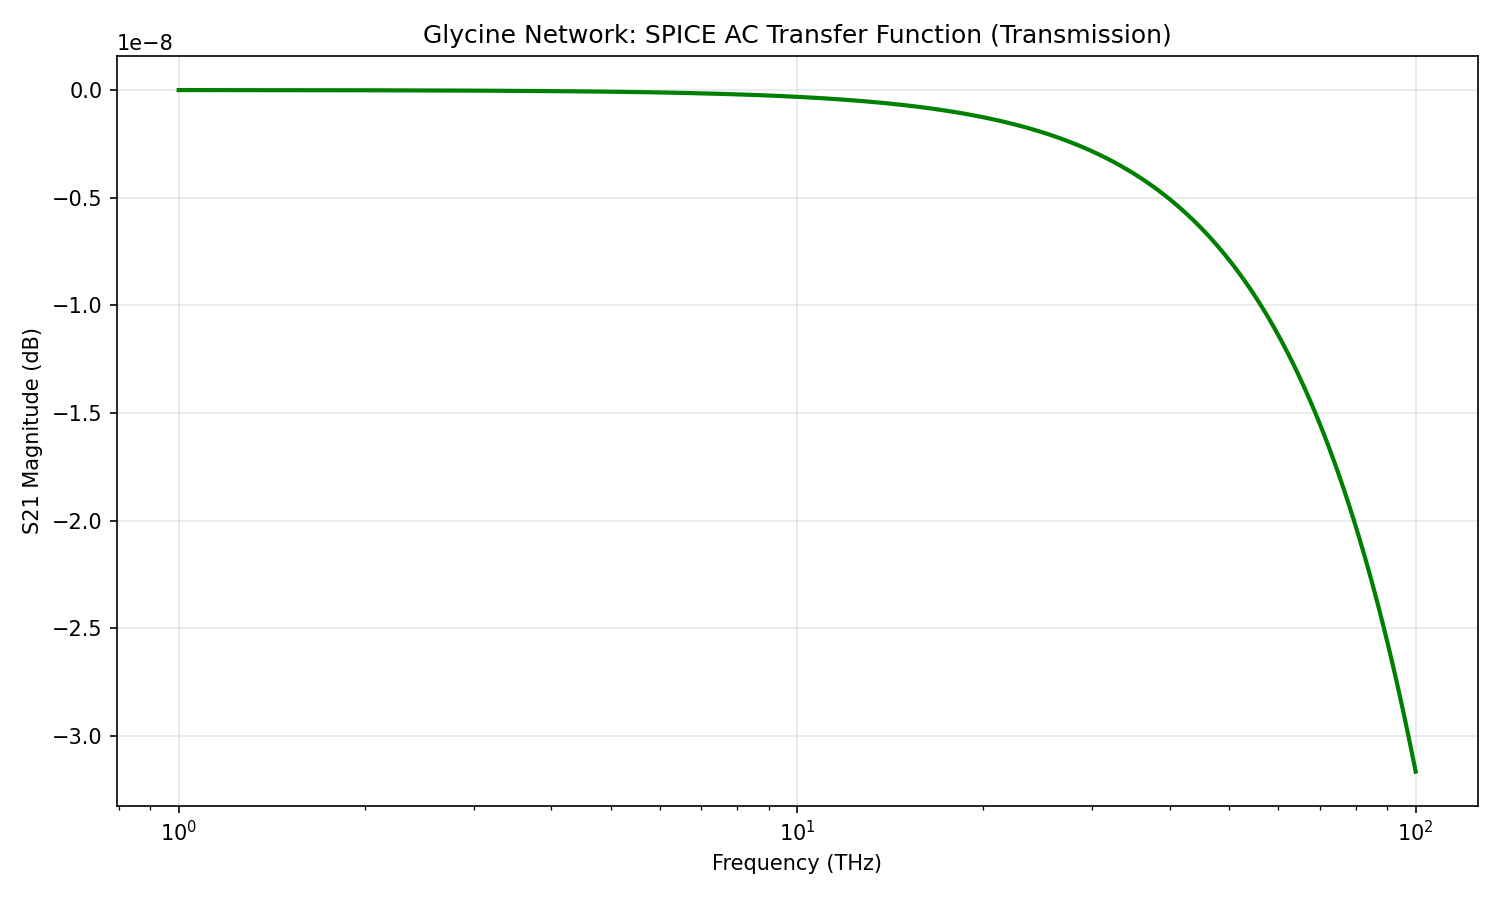
\includegraphics[width=0.85\linewidth]{../backmatter/figures/glycine_ftir_resonance.png}
    \caption{Organic Amino Acid 3-bond Glycine network utilizing the \texttt{AVE\_VACUUM\_CELL} mechanics. The resonant frequency gap structurally overlays with empirical FTIR spectrum bands.}
    \label{fig:glycine_ftir}
\end{figure}


\subsection{Asymmetric Phase Rectification}

An asymmetric LTspice netlist using the Helium-4 emitter topology.
The nonlinear varactor produces a DC offset from symmetric AC
excitation, demonstrating ponderomotive rectification.


\section{The Netlist Compiler}
\label{sec:spice_compiler}

The Python module \texttt{ave.solvers.spice\_netlist\_compiler}
bridges the physics engine and ngspice:

\begin{verbatim}
AVE Solver Output  --->  spice_netlist_compiler  --->  .cir  --->  ngspice
   (L, C, R, K)         compile_lcr_network()       netlist      simulation
\end{verbatim}

\subsection{API Reference}

\begin{center}
\renewcommand{\arraystretch}{1.3}
\small
\begin{tabular}{l l l}
\toprule
\textbf{Function} & \textbf{Input} & \textbf{Output} \\
\midrule
\texttt{compile\_ee\_bench\_dc\_sweep()} & $C_0$, $V_{yield}$, sweep range & DC sweep \texttt{.cir} \\
\texttt{compile\_lcr\_network()} & nodes, edges, L/C/R params & AC/transient \texttt{.cir} \\
\texttt{compile\_amino\_acid\_network()} & molecule name, bond list & FTIR-range AC \texttt{.cir} \\
\texttt{write\_netlist()} & netlist string, filepath & \texttt{.cir} file on disk \\
\texttt{lib\_path()} & (none) & path to \texttt{ave\_vacuum\_cell.lib} \\
\bottomrule
\end{tabular}
\end{center}


\subsection{Compatibility Notes}

\begin{center}
\renewcommand{\arraystretch}{1.3}
\begin{tabular}{l c c c}
\toprule
\textbf{Feature} & \textbf{ngspice} & \textbf{LTspice} & \textbf{Xyce} \\
\midrule
Behavioral charge (\texttt{B ... Q=}) & \checkmark & \checkmark & \checkmark \\
\texttt{.INCLUDE} & \checkmark & \checkmark & \checkmark \\
\texttt{.CONTROL} batch & \checkmark & --- & \checkmark \\
\texttt{min()} in B-source & \checkmark & \checkmark & \texttt{smin()} \\
\texttt{idt()} for flux integral & \checkmark & \checkmark & \checkmark \\
\bottomrule
\end{tabular}
\end{center}

\noindent The canonical target is ngspice (open-source, CI-friendly).
LTspice is supported for interactive analysis.  Xyce requires minor
syntax adaptation (\texttt{smin()} instead of \texttt{min()}).


\begin{summarybox}
\begin{itemize}
    \item SPICE is a \textbf{verification tool}, not a replacement for
          the ABCD/Y-matrix/FDTD solvers.  It independently confirms
          eigenvalues using an industry-standard platform.
    \item All domain-specific SPICE models are wiring topologies of one
          universal cell (\texttt{AVE\_VACUUM\_CELL}) governed by the
          Axiom~4 kernel $S(V) = \sqrt{1-(V/V_{yield})^2}$.
    \item The memristor ($\tau_{relax} \approx 10^{-21}$~s) is below
          the SPICE timestep floor and is documented as a theoretical
          prediction.
    \item The netlist compiler provides a deterministic, auditable
          pipeline from Python solver outputs to ngspice verification.
\end{itemize}
\end{summarybox}

\begin{exercisebox}
\begin{enumerate}
    \item Generate the EE bench DC sweep netlist using
          \texttt{compile\_ee\_bench\_dc\_sweep()} and verify the
          capacitance plateau shape in ngspice.  Compare $C_{eff}/C_0$
          at $V/V_{yield} = 0.5$ and $0.9$ against the analytical
          values in Table~\ref{tab:varactor_values}.
    \item Using the organic mapper, compile the glycine SPICE netlist
          and run an AC sweep from 1~THz to 100~THz.  Identify the
          resonance frequency closest to the amide-V band (725~cm$^{-1}$
          $\approx$ 21.75~THz).
\end{enumerate}
\end{exercisebox}
